\section{Business Relationships with Neighbouring ISPs}
\label{sec:relationships}

BT Network has three immediate neighbouring ISPs and it's important to form business relationships with all three of them in order to gain economic benefits. 
The external routing policies of BGP protocol for each outside network are determined by its business relationship with us (see Section \ref{sec:bgp} for details).
Business relationships with neighbouring ISPs are shown in Figure \ref{fig:relationships} and elaborated in the following.

\begin{figure*}[ht!]
    \centering
    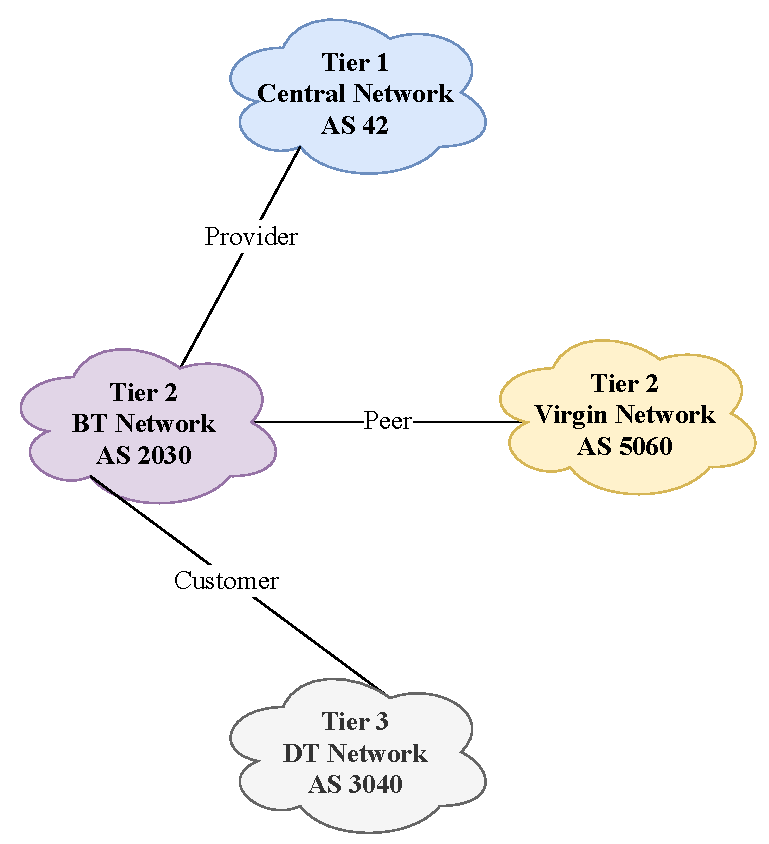
\includegraphics[width=0.5\linewidth]{relationships}
    \caption{Business Relationships of BT Network with Neighbouring ISPs.}
    \label{fig:relationships}
\end{figure*}


\subsection{Provider: Central Network}
Since BT Network is a Tier-2 ISP, it need to be connected to a Tier-1 ISP to gain broader Internet connection. Therefore, BT is connected to Central Network, a Tier-1 ISP, as a customer which makes it a network provider for BT.

\subsection{Peer: Virgin Network}
BT Network forms a Peer relationship with Virgin Network. This allows Virgin Network to connect to BT Network at zero cost and vice versa.

\subsection{Customer: DT Network}
\label{sec:dt}
BT Network forms a Provider-Customer relationship with DT Network, in which BT is the provider and DT is the customer. In other words, DT gains access to the broader Internet through BT at a cost.
